\subsection{Nuclear LWR, China and India (3,150~\$/kW)}\label{sec:nuclear-lwr-cnin}

Recent project data show that China and India build light- and heavy-water reactors at lower cost than other countries, and the West in particular (Figure~\ref{fig:nuclear-strip}), so we give them their own cost bin.
The usual explanation is that both countries build in series, with dedicated crews moving from site to site.

Audited final costs are rarely published there, so ex-post construction costs are largely unavailable.
We therefore scale the available ex-ante figures by 1.27, the median ratio of final (or latest) to initial estimate over all projects in our dataset that report both.

\begin{figure}[htbp]\centering
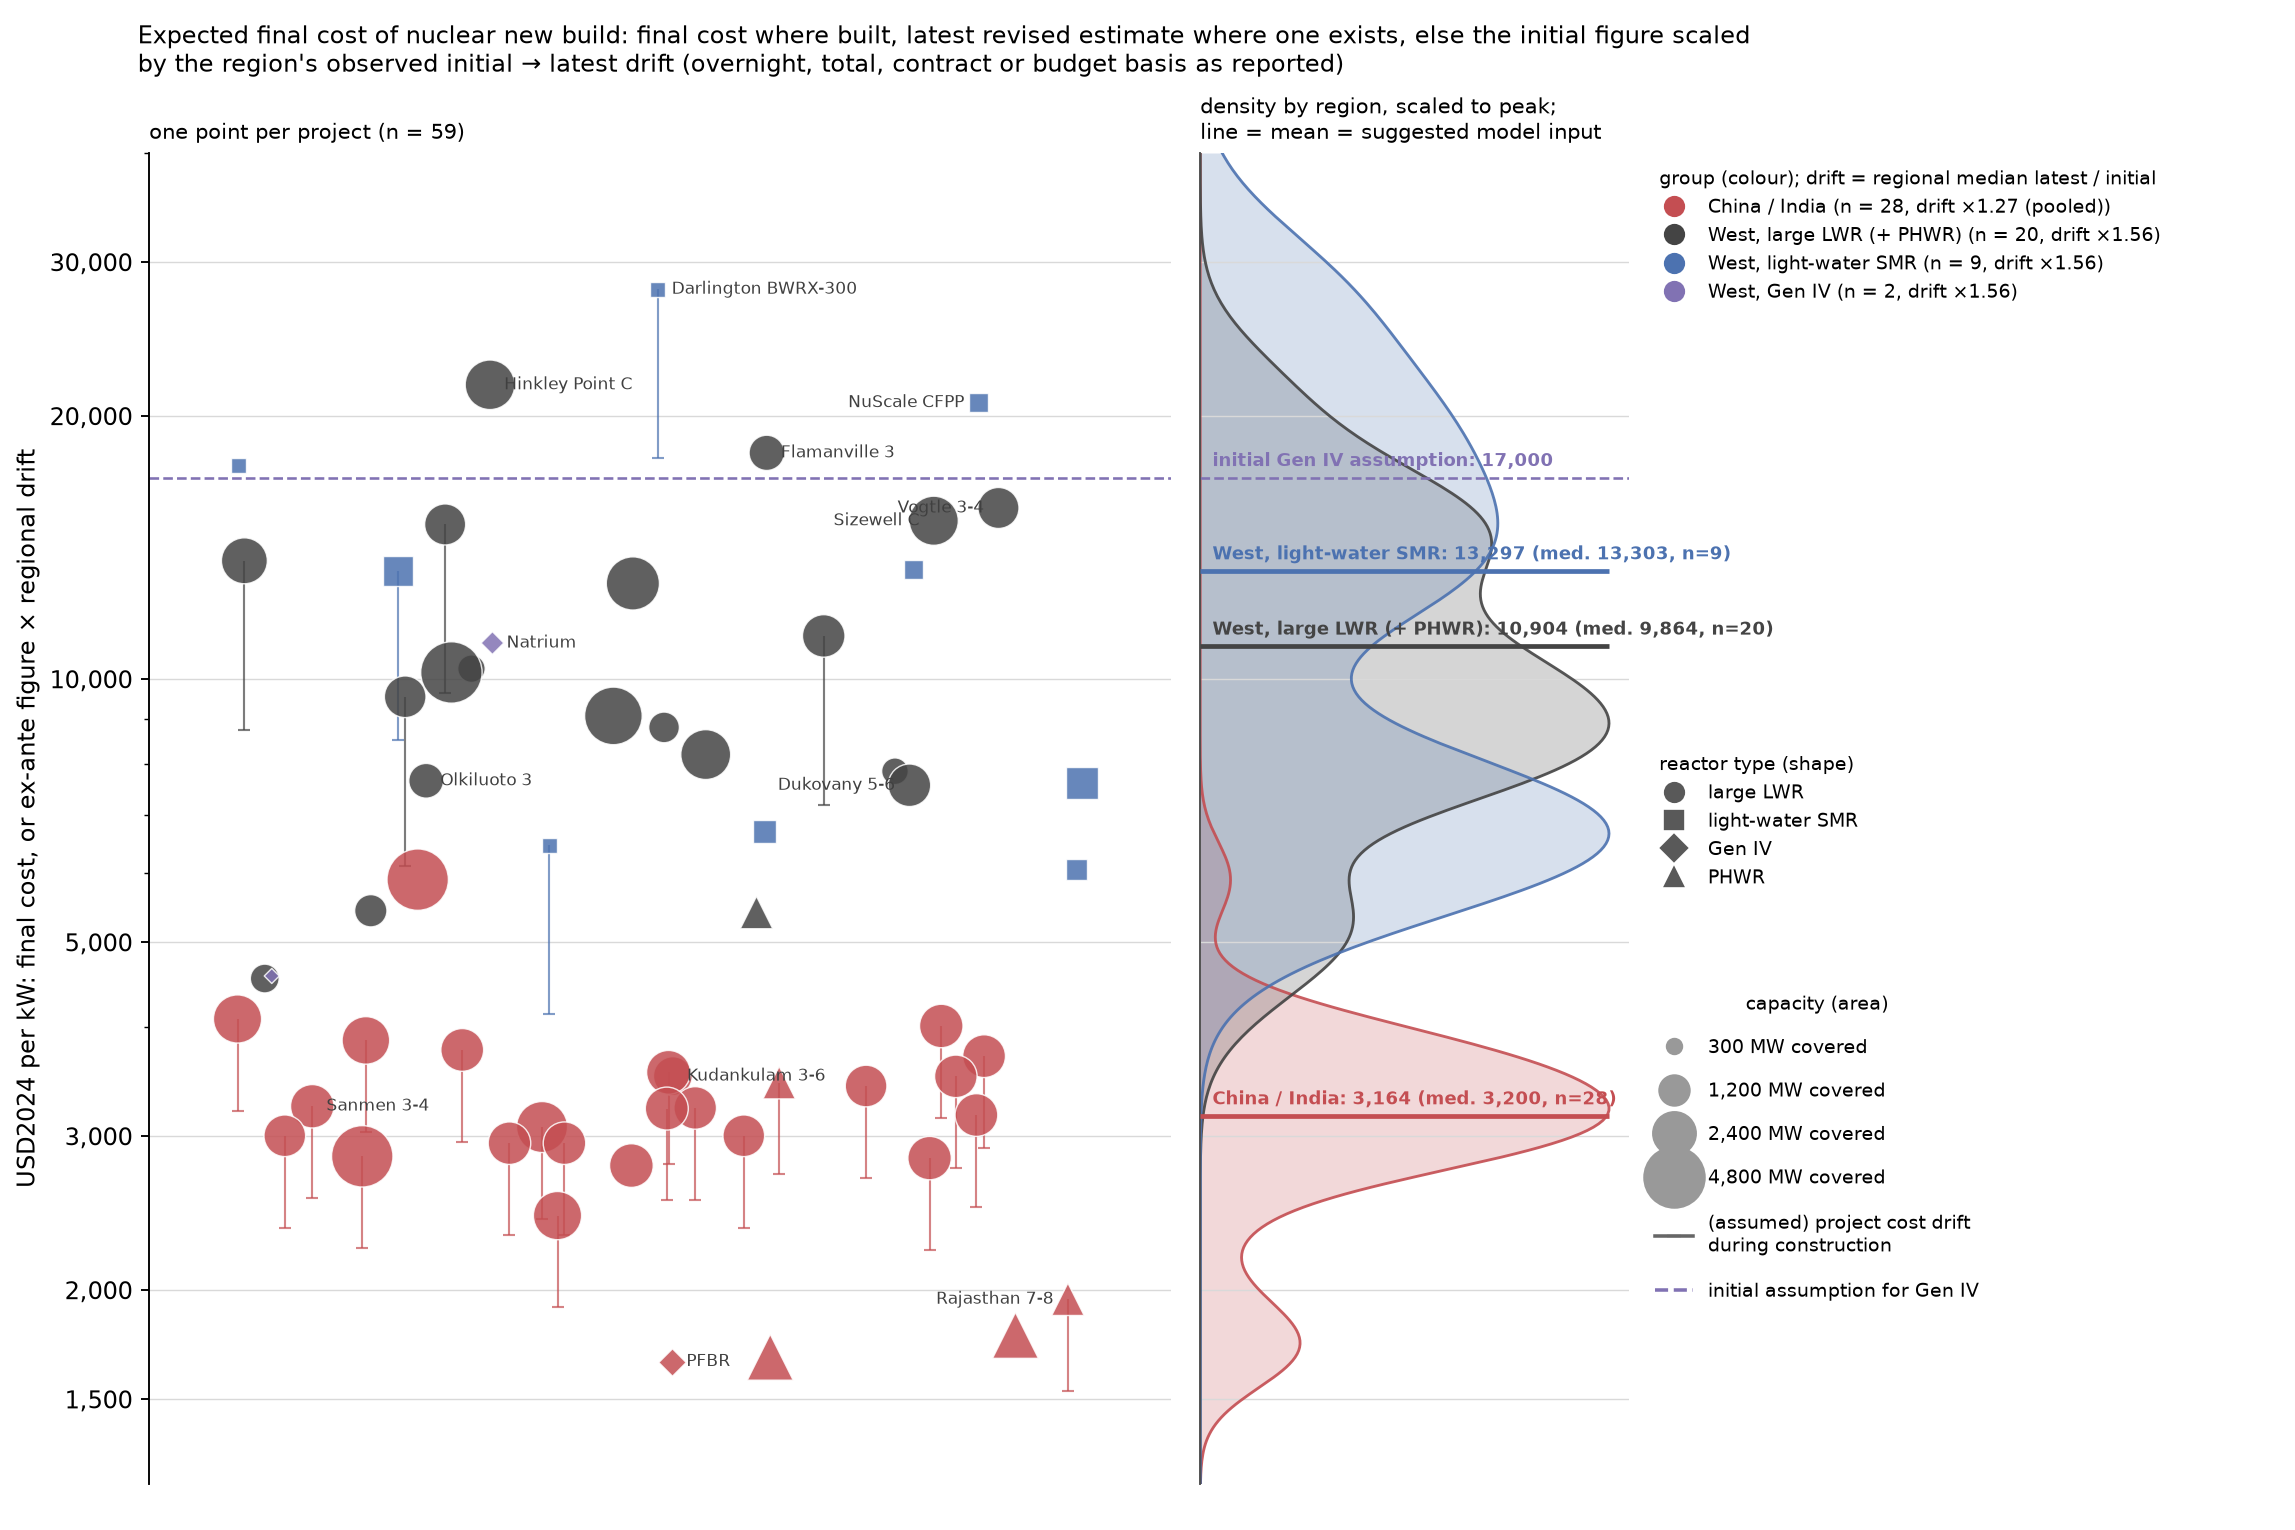
\includegraphics[width=\textwidth]{../../../misc-quarter1/nuclear-projects/figures/nuclear_cost_strip.png}
\caption{
  Expected final cost per kW of nuclear projects with a published figure, by region and reactor type:
  final cost where built, latest estimate where available, otherwise the initial estimate is scaled by the observed regional drift.
  One point per project; vertical lines lead from the initial estimate to the expected final cost.
  The points are 59 projects compiled from public sources, each with its source in \texttt{misc-quarter1/nuclear-projects/data/project\_costs.csv}; unit data from the GEM tracker \citep{gem2026}.
}
\label{fig:nuclear-strip}
\end{figure}

Based on these projects, we use 3,150~\$/kW (median 3,200; Figure~\ref{fig:nuclear-strip}).
For simplicity, large reactors and SMRs share the bin.

The learning rate is zero.
Both countries build reactors in series and their costs have been flat since 2010, so there is no evidence for further learning.

O\&M cost, efficiency and the 60-year lifetime come from technology-data's nuclear entry \citep{technologydata}.
The fuel price of 2~\$/MWh\textsubscript{th}, about 6~\$ per MWh of electricity, follows from US plants, where fuel makes up 15--20\,\% of a generating cost of about 31~\$/MWh \citep{doe2024nuclear}; technology-data's 8.2~\$/MWh\textsubscript{th} is four times higher.
The lead time of 6~years is China's median build time \citep{gem2026}.

Without a build limit, the model would build excessive nuclear capacity in China and India.
Construction currently starts at about 10~GW/yr in China (11~GW in 2025) and 2~GW/yr in India \citep{gem2026};
we carry these into the model, and show for representation their sum 12~GW/yr in this document's Table~\ref{tab:deployment}.
